\documentclass[12pt,a4paper,twoside]{report}

% ============================================
% PACKAGES
% ============================================
\usepackage[utf8]{inputenc}
\usepackage[T1]{fontenc}
\usepackage[french]{babel}
\usepackage{geometry}
\usepackage{graphicx}
\usepackage{xcolor}
\usepackage{hyperref}
\usepackage{fancyhdr}
\usepackage{titlesec}
\usepackage{booktabs}
\usepackage{array}
\usepackage{longtable}
\usepackage{colortbl}
\usepackage{listings}
\usepackage{tcolorbox}
\usepackage{enumitem}
\usepackage{tikz}
\usepackage{float}
\usepackage{caption}
\usepackage{subcaption}
\usepackage{setspace}
\usepackage{amsmath}
\usepackage{amssymb}
\usepackage{pdfpages}
\usepackage{appendix}
\usepackage{tocloft}
\usepackage{etoolbox}
\usepackage{csquotes}

% ============================================
% PAGE GEOMETRY
% ============================================
\geometry{
    a4paper,
    left=2.5cm,
    right=2.5cm,
    top=2.5cm,
    bottom=2.5cm
}

% ============================================
% COLORS
% ============================================
\definecolor{orange}{HTML}{FF6600}
\definecolor{orangedark}{HTML}{CC5200}
\definecolor{darkblue}{HTML}{003366}
\definecolor{lightgray}{HTML}{F5F5F5}
\definecolor{codebg}{HTML}{F8F8F8}
\definecolor{codeframe}{HTML}{CCCCCC}

% ============================================
% HYPERREF SETUP
% ============================================
\hypersetup{
    colorlinks=true,
    linkcolor=darkblue,
    urlcolor=orange,
    citecolor=darkblue,
    pdftitle={Plateforme Cloud OSS - Orange Tunisie},
    pdfauthor={Auteur}
}

% ============================================
% HEADER/FOOTER
% ============================================
\pagestyle{fancy}
\fancyhf{}
\fancyhead[LE,RO]{\thepage}
\fancyhead[RE]{\leftmark}
\fancyhead[LO]{\rightmark}
\renewcommand{\headrulewidth}{0.4pt}
\renewcommand{\footrulewidth}{0pt}

% ============================================
% CHAPTER/SECTION FORMATTING
% ============================================
\titleformat{\chapter}[display]
    {\normalfont\huge\bfseries\color{orange}}
    {\chaptertitlename\ \thechapter}{20pt}{\Huge}
    
\titleformat{\section}
    {\Large\bfseries\color{darkblue}}
    {\thesection}{1em}{}
    
\titleformat{\subsection}
    {\large\bfseries\color{darkblue}}
    {\thesubsection}{1em}{}

\titleformat{\subsubsection}
    {\normalsize\bfseries}
    {\thesubsubsection}{1em}{}

% ============================================
% CODE LISTING STYLE
% ============================================
\lstset{
    basicstyle=\ttfamily\small,
    backgroundcolor=\color{codebg},
    frame=single,
    rulecolor=\color{codeframe},
    breaklines=true,
    showstringspaces=false,
    columns=flexible,
    numbers=left,
    numberstyle=\tiny\color{gray},
    keywordstyle=\color{blue},
    commentstyle=\color{green!50!black},
    stringstyle=\color{red},
    tabsize=4
}

% ============================================
% CUSTOM BOXES
% ============================================
\tcbuselibrary{skins,breakable}

\newtcolorbox{infobox}[1][]{
    colback=blue!5,
    colframe=blue!50,
    title=#1,
    breakable
}

\newtcolorbox{warningbox}[1][]{
    colback=orange!5,
    colframe=orange,
    title=#1,
    breakable
}

% ============================================
% LINE SPACING
% ============================================
\onehalfspacing

% ============================================
% DOCUMENT START
% ============================================
\begin{document}

% ============================================
% PAGE DE GARDE
% ============================================
\begin{titlepage}
    % Background avec triangles géométriques
    \begin{tikzpicture}[remember picture, overlay]
        % Triangles gris (gauche)
        \fill[gray!40] (current page.north west) -- ++(0,-6) -- ++(3,0) -- cycle;
        \fill[gray!30] (current page.north west) ++ (0,-4) -- ++(0,-5) -- ++(4,0) -- cycle;
        \fill[gray!50] (current page.north west) ++ (0,-8) -- ++(0,-4) -- ++(2.5,0) -- cycle;
        \fill[gray!25] (current page.north west) ++ (0,-11) -- ++(0,-6) -- ++(5,0) -- cycle;
        \fill[gray!35] (current page.north west) ++ (0,-15) -- ++(0,-5) -- ++(3,0) -- cycle;
        
        % Triangles rouges/orange
        \fill[orange!80] (current page.north west) ++ (2,-3) -- ++(0,-3) -- ++(2,0) -- cycle;
        \fill[red!70] (current page.north west) ++ (1,-7) -- ++(0,-2.5) -- ++(2,0) -- cycle;
        \fill[orange!60] (current page.north west) ++ (3,-10) -- ++(0,-3) -- ++(2.5,0) -- cycle;
        \fill[red!60] (current page.north west) ++ (0.5,-13) -- ++(0,-2) -- ++(1.5,0) -- cycle;
        \fill[orange!70] (current page.north west) ++ (2,-16) -- ++(0,-2.5) -- ++(2,0) -- cycle;
        
        % Petits triangles décoratifs
        \fill[gray!60] (current page.north west) ++ (4,-5) -- ++(0,-1.5) -- ++(1,0) -- cycle;
        \fill[red!50] (current page.north west) ++ (3.5,-12) -- ++(0,-1.5) -- ++(1.2,0) -- cycle;
        \fill[gray!45] (current page.north west) ++ (1.5,-18) -- ++(0,-2) -- ++(1.5,0) -- cycle;
        
        % Cadre rouge pour le diplôme
        \draw[red!80, line width=2pt] ([xshift=2cm, yshift=-8.5cm]current page.north) rectangle ++(13,1.2);
    \end{tikzpicture}
    
    \centering
    
    % Logo ESPRIT
    
\includegraphics[width=5cm]{images/img-000.png}
    
    \vspace{0.8cm}
    
    {\Large\bfseries\textcolor{orange}{2024 - 2025}}
    
    \vspace{0.3cm}
    
    {\large PROJET DE FIN D'ÉTUDES}
    
    \vspace{0.8cm}
    
    \rule{0.9\textwidth}{1.5pt}
    
    \vspace{0.5cm}
    
    {\Large\bfseries DIPLÔME NATIONAL D'INGÉNIEUR}
    
    \vspace{0.3cm}
    
    {\large SPÉCIALITÉ : INFORMATIQUE}
    
    \vspace{0.5cm}
    
    \rule{0.9\textwidth}{1.5pt}
    
    \vspace{1cm}
    
    {\LARGE\bfseries Mise en œuvre d'une solution}
    
    \vspace{0.2cm}
    
    {\LARGE\bfseries automatisée sur un cloud privé pour}
    
    \vspace{0.2cm}
    
    {\LARGE\bfseries l'orchestration des workflow OSS}
    
    \vspace{1.5cm}
    
    \begin{minipage}{0.45\textwidth}
        \begin{flushleft}
            \textbf{Réalisé par :}\\
            Nom Prénom
        \end{flushleft}
    \end{minipage}
    \hfill
    \begin{minipage}{0.45\textwidth}
        \begin{flushright}
            \textbf{Encadrant entreprise :}\\
            Nom Encadrant
        \end{flushright}
    \end{minipage}
    
    \vspace{0.8cm}
    
    \begin{minipage}{0.45\textwidth}
        \begin{flushleft}
            \textbf{Encadrant académique :}\\
            Nom Encadrant Académique
        \end{flushleft}
    \end{minipage}
    
    \vfill
    
    % Logos en bas de page
    \begin{minipage}{\textwidth}
        \centering
        \begin{tabular}{ccccc}
            
\includegraphics[height=1.2cm]{images/img-001.png} &
            \hspace{0.5cm} &
            
\includegraphics[height=1.2cm]{images/img-002.png} &
            \hspace{0.5cm} &
            
\includegraphics[height=1.2cm]{images/img-004.png}
        \end{tabular}
    \end{minipage}
    
\end{titlepage}

% ============================================
% PAGES LIMINAIRES
% ============================================
\pagenumbering{roman}

% Dédicaces
\chapter*{Dédicaces}
\addcontentsline{toc}{chapter}{Dédicaces}

\begin{center}
\textit{À mes parents,\\
À ma famille,\\
À mes amis}
\end{center}

\newpage

% Remerciements
\chapter*{Remerciements}
\addcontentsline{toc}{chapter}{Remerciements}

Je tiens à remercier toutes les personnes qui ont contribué à la réalisation de ce projet de fin d'études.

Je remercie particulièrement mon encadrant pour ses conseils précieux et son accompagnement tout au long de ce travail.

Je remercie également l'équipe d'Orange Tunisie pour leur accueil chaleureux et leur soutien technique.

\newpage

% Table des matières
\tableofcontents
\newpage

% Liste des figures
\listoffigures
\addcontentsline{toc}{chapter}{Table des figures}
\newpage

% Liste des tableaux
\listoftables
\addcontentsline{toc}{chapter}{Liste des tableaux}
\newpage

% Liste des abréviations
\chapter*{Liste des abréviations}
\addcontentsline{toc}{chapter}{Liste des abréviations}

\begin{tabular}{ll}
    \textbf{API} & Application Programming Interface \\
    \textbf{CI/CD} & Continuous Integration / Continuous Deployment \\
    \textbf{DevOps} & Development and Operations \\
    \textbf{DevSecOps} & Development, Security and Operations \\
    \textbf{IaaS} & Infrastructure as a Service \\
    \textbf{K8s} & Kubernetes \\
    \textbf{OSS} & Operations Support System \\
    \textbf{PaaS} & Platform as a Service \\
    \textbf{RBAC} & Role-Based Access Control \\
    \textbf{SaaS} & Software as a Service \\
    \textbf{VM} & Virtual Machine \\
    \textbf{WAF} & Web Application Firewall \\
\end{tabular}

\newpage

% ============================================
% CONTENU PRINCIPAL
% ============================================
\pagenumbering{arabic}

% Introduction Générale
\chapter*{Introduction Générale}
\addcontentsline{toc}{chapter}{Introduction Générale}

Dans un contexte de transformation numérique accélérée, les opérateurs télécom comme Orange Tunisie font face à des défis majeurs en matière de gestion de leur infrastructure IT et de leurs systèmes d'exploitation (OSS - Operations Support Systems).

Ce projet de fin d'études vise à concevoir et déployer une plateforme cloud complète intégrant :
\begin{itemize}
    \item \textbf{OpenStack} pour la virtualisation de l'infrastructure
    \item \textbf{Kubernetes} pour l'orchestration des conteneurs
    \item \textbf{DevSecOps} pour l'automatisation sécurisée des déploiements
    \item \textbf{Offres B2B} (IaaS, PaaS, SaaS) pour les clients entreprises
\end{itemize}

Le document est organisé en six chapitres couvrant l'ensemble du cycle de développement selon la méthodologie Scrum.

\newpage

% ============================================
% CHAPITRE 1
% ============================================
\chapter{Cadre Initial et Préparation du Projet}

\section{Présentation de l'organisation d'accueil}

\subsection{Orange Tunisie}

Orange Tunisie est l'un des principaux opérateurs de télécommunications en Tunisie, offrant une gamme complète de services mobiles, fixes et Internet. Fondée en 2002, l'entreprise s'est imposée comme un acteur majeur du secteur.

\begin{figure}[H]
    \centering
    
\includegraphics[width=0.3\textwidth]{images/img-002.png}
    \caption{Logo Orange}
    \label{fig:logo-orange}
\end{figure}

\subsection{Domaines d'activités}

Orange Tunisie opère dans plusieurs domaines :
\begin{itemize}
    \item \textbf{Téléphonie mobile} : Services voix, SMS, données
    \item \textbf{Internet fixe} : ADSL, fibre optique
    \item \textbf{Solutions entreprises} : Cloud, cybersécurité, IoT
    \item \textbf{Services financiers} : Orange Money
\end{itemize}

\subsection{Structure organisationnelle}

\begin{figure}[H]
    \centering
    
\includegraphics[width=0.8\textwidth]{images/img-003.png}
    \caption{Organigramme de l'organisme d'accueil}
    \label{fig:organigramme}
\end{figure}

\section{Contexte du projet}

Le projet s'inscrit dans la stratégie de modernisation des infrastructures IT d'Orange Tunisie, visant à :
\begin{itemize}
    \item Centraliser et automatiser la gestion des OSS
    \item Adopter une approche cloud-native
    \item Proposer des services B2B compétitifs
\end{itemize}

\section{Problématique, analyse de l'existant et solutions proposées}

\subsection{Problématique}

Comment centraliser et automatiser la gestion des différents OSS tout en assurant leur sécurité et en proposant des services cloud aux clients B2B ?

\subsection{Analyse de l'Existant}

L'infrastructure existante présente plusieurs limitations :
\begin{itemize}
    \item Silos technologiques entre les différents OSS
    \item Processus manuels et répétitifs
    \item Manque de visibilité sur les performances
    \item Absence d'offres cloud standardisées
\end{itemize}

\subsection{Solutions Proposées}

\begin{figure}[H]
    \centering
    
\includegraphics[width=0.9\textwidth]{images/img-005.png}
    \caption{Architecture de la plateforme OSS proposée}
    \label{fig:architecture-proposee}
\end{figure}

La solution proposée repose sur :
\begin{enumerate}
    \item \textbf{OpenStack} : Couche IaaS pour la virtualisation
    \item \textbf{Kubernetes} : Orchestration des conteneurs
    \item \textbf{Rancher} : Gestion multi-cluster
    \item \textbf{GitLab CI/CD} : Automatisation des déploiements
    \item \textbf{Prometheus/Grafana} : Monitoring et alerting
\end{enumerate}

\section{Méthodologie de travail agile (Scrum)}

\subsection{Choix de la méthode}

Scrum a été choisie pour sa flexibilité et son adaptabilité aux projets complexes.

\subsection{Comparatif des méthodologies}

\begin{table}[H]
    \centering
    \caption{Comparatif des méthodologies agiles}
    \label{tab:methodologies}
    \rowcolors{2}{lightgray}{white}
    \begin{tabular}{|l|c|c|c|}
        \hline
        \rowcolor{orange!80}
        \textcolor{white}{\textbf{Critère}} & \textcolor{white}{\textbf{Scrum}} & \textcolor{white}{\textbf{Kanban}} & \textcolor{white}{\textbf{XP}} \\
        \hline
        Itérations fixes & Oui & Non & Oui \\
        Rôles définis & Oui & Non & Oui \\
        Flexibilité & Moyenne & Haute & Faible \\
        Documentation & Légère & Minimale & Minimale \\
        \hline
    \end{tabular}
\end{table}

\subsection{Organisation du projet en sprints Scrum}

Le projet est organisé en 8 sprints de 2-3 semaines chacun :

\begin{table}[H]
    \centering
    \caption{Planning des sprints}
    \label{tab:sprints}
    \rowcolors{2}{lightgray}{white}
    \begin{tabular}{|c|l|l|}
        \hline
        \rowcolor{orange!80}
        \textcolor{white}{\textbf{Sprint}} & \textcolor{white}{\textbf{Objectif}} & \textcolor{white}{\textbf{Durée}} \\
        \hline
        1 & Étude préliminaire et choix technologiques & 2 semaines \\
        2 & Automatisation Cloud (OpenStack) & 3 semaines \\
        3 & Orchestration workflows (Camunda) & 3 semaines \\
        4 & Monitoring (Prometheus/Grafana) & 2 semaines \\
        5 & CI/CD et gouvernance & 3 semaines \\
        6 & Sécurité (KubeHunter, Graylog) & 2 semaines \\
        7 & Interface utilisateur & 3 semaines \\
        8 & Offres B2B (IaaS, PaaS, SaaS) & 3 semaines \\
        \hline
    \end{tabular}
\end{table}

\newpage

% ============================================
% CHAPITRE 2
% ============================================
\chapter{Étude Préliminaire et Choix Technologiques (Sprint 1)}

\section{Workflow OSS}

\subsection{Orchestration de workflow OSS}

L'orchestration des workflows OSS permet de coordonner les différentes tâches et processus de manière automatisée.

\subsection{Centralisation de workflow OSS}

La centralisation permet d'avoir une vue unifiée de tous les processus OSS.

\subsection{Supervision et Sécurisation de workflow OSS}

La supervision en temps réel et la sécurisation des workflows sont essentielles pour garantir la disponibilité des services.

\section{Le Cloud Computing chez Orange}

Orange adopte une stratégie multi-cloud avec :
\begin{itemize}
    \item Cloud privé basé sur OpenStack
    \item Cloud public pour certains services
    \item Cloud hybride pour la flexibilité
\end{itemize}

\begin{figure}[H]
    \centering
    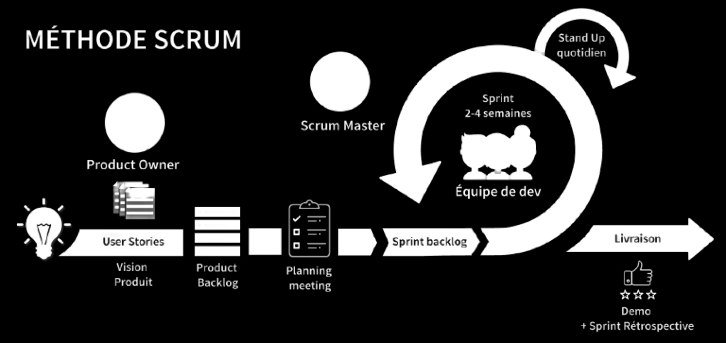
\includegraphics[width=0.6\textwidth]{images/img-008.png}
    \caption{Modèle de cloud}
    \label{fig:cloud-model}
\end{figure}

\section{DevOps et DevSecOps}

\begin{figure}[H]
    \centering
    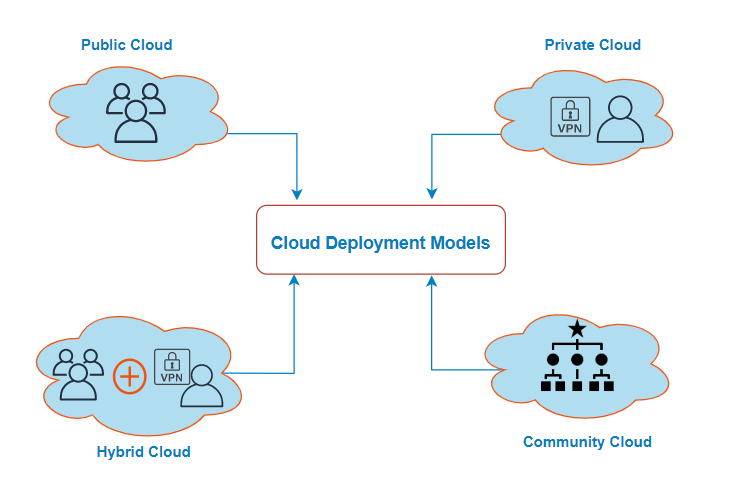
\includegraphics[width=0.7\textwidth]{images/img-009.png}
    \caption{DevSecOps}
    \label{fig:devsecops}
\end{figure}

Le DevSecOps intègre la sécurité dès les premières phases du développement.

\section{Technologies Retenues}

\subsection{Outils d'Infrastructure}

\subsubsection{OpenStack}

\begin{figure}[H]
    \centering
    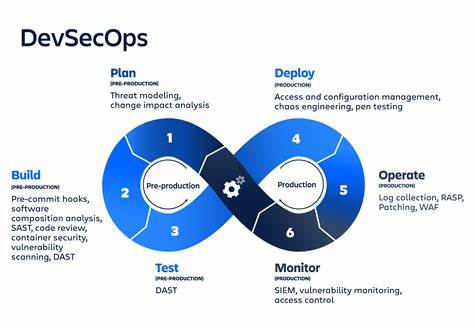
\includegraphics[width=0.4\textwidth]{images/img-010.png}
    \caption{OpenStack}
    \label{fig:openstack}
\end{figure}

OpenStack est une plateforme open source de cloud computing IaaS.

\subsubsection{Kubernetes}

\begin{figure}[H]
    \centering
    
\includegraphics[width=0.3\textwidth]{images/img-011.png}
    \caption{Kubernetes}
    \label{fig:kubernetes}
\end{figure}

Kubernetes (K8s) est un système d'orchestration de conteneurs.

\subsubsection{Rancher}

\begin{figure}[H]
    \centering
    
\includegraphics[width=0.3\textwidth]{images/img-012.png}
    \caption{Rancher}
    \label{fig:rancher}
\end{figure}

Rancher facilite la gestion de clusters Kubernetes multiples.

\subsection{Outils d'Automatisation}

\subsubsection{Terraform}

\begin{figure}[H]
    \centering
    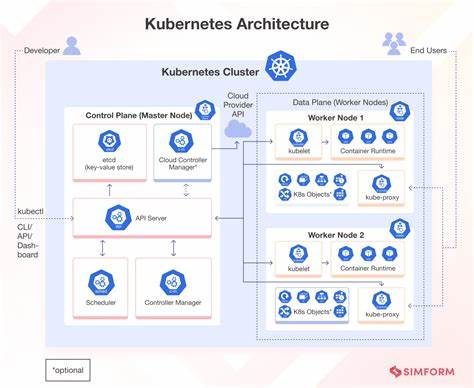
\includegraphics[width=0.3\textwidth]{images/img-013.png}
    \caption{Terraform}
    \label{fig:terraform}
\end{figure}

Terraform permet l'Infrastructure as Code (IaC).

\subsubsection{Ansible}

\begin{figure}[H]
    \centering
    
\includegraphics[width=0.3\textwidth]{images/img-014.png}
    \caption{Ansible}
    \label{fig:ansible}
\end{figure}

Ansible automatise la configuration et le déploiement.

\subsection{Outil d'Orchestration : Camunda}

\begin{figure}[H]
    \centering
    
\includegraphics[width=0.3\textwidth]{images/img-015.png}
    \caption{Camunda}
    \label{fig:camunda}
\end{figure}

Camunda est un moteur BPMN pour l'orchestration des processus métier.

\subsection{Outils de Sécurité}

\subsubsection{Trivy}

\begin{figure}[H]
    \centering
    
\includegraphics[width=0.3\textwidth]{images/img-016.png}
    \caption{Trivy}
    \label{fig:trivy}
\end{figure}

Scanner de vulnérabilités pour images Docker.

\subsubsection{KubeHunter}

\begin{figure}[H]
    \centering
    
\includegraphics[width=0.3\textwidth]{images/img-017.png}
    \caption{KubeHunter}
    \label{fig:kubehunter}
\end{figure}

Outil de pentest pour clusters Kubernetes.

\subsection{Outils de Monitoring et Logs}

\subsubsection{Prometheus et Grafana}

\begin{figure}[H]
    \centering
    
\includegraphics[width=0.5\textwidth]{images/img-018.png}
    \caption{Prometheus et Grafana}
    \label{fig:prometheus-grafana}
\end{figure}

Stack de monitoring et visualisation.

\subsubsection{Graylog}

\begin{figure}[H]
    \centering
    
\includegraphics[width=0.3\textwidth]{images/img-019.png}
    \caption{Graylog}
    \label{fig:graylog}
\end{figure}

Centralisation et analyse des logs.

\subsection{Outils de Tests et Qualité}

\subsubsection{K6}

\begin{figure}[H]
    \centering
    
\includegraphics[width=0.3\textwidth]{images/img-020.png}
    \caption{K6}
    \label{fig:k6}
\end{figure}

Outil de tests de charge.

\subsubsection{SonarQube}

\begin{figure}[H]
    \centering
    
\includegraphics[width=0.3\textwidth]{images/img-021.png}
    \caption{SonarQube}
    \label{fig:sonarqube}
\end{figure}

Analyse de qualité du code.

\subsection{Outil de Gestion API : WSO2}

\begin{figure}[H]
    \centering
    
\includegraphics[width=0.3\textwidth]{images/img-022.png}
    \caption{WSO2}
    \label{fig:wso2}
\end{figure}

\subsection{Outil CI/CD : GitLab}

\begin{figure}[H]
    \centering
    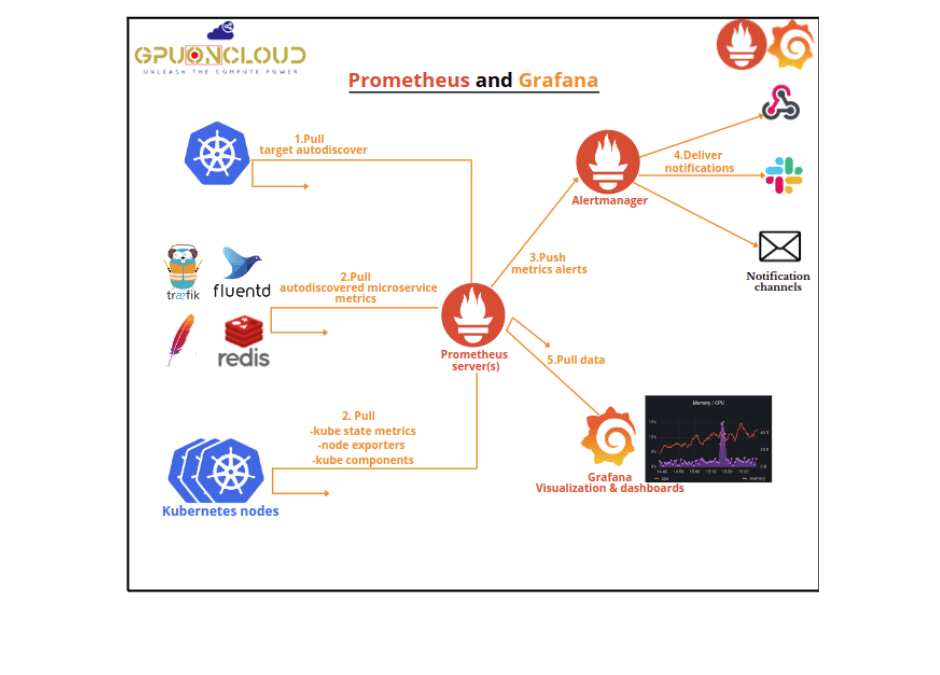
\includegraphics[width=0.3\textwidth]{images/img-023.png}
    \caption{GitLab}
    \label{fig:gitlab}
\end{figure}

GitLab CI/CD pour l'intégration et le déploiement continus.

\newpage

% ============================================
% CHAPITRE 3
% ============================================
\chapter{Analyse des besoins et cadre fonctionnel (Sprint 1)}

\section{Identification des parties prenantes}

\begin{table}[H]
    \centering
    \caption{Parties prenantes du projet}
    \label{tab:parties-prenantes}
    \rowcolors{2}{lightgray}{white}
    \begin{tabular}{|l|p{8cm}|}
        \hline
        \rowcolor{orange!80}
        \textcolor{white}{\textbf{Acteur}} & \textcolor{white}{\textbf{Rôle}} \\
        \hline
        Administrateur & Gestion de la plateforme et des utilisateurs \\
        Utilisateur interne & Utilisation opérationnelle des services \\
        Auditeur sécurité & Audit et conformité \\
        Client B2B & Consommation des services IaaS/PaaS/SaaS \\
        \hline
    \end{tabular}
\end{table}

\section{Objectifs fonctionnels du système}

\begin{itemize}
    \item Centraliser la gestion des OSS
    \item Automatiser les déploiements CI/CD
    \item Sécuriser l'infrastructure
    \item Proposer des offres B2B
    \item Monitorer en temps réel
\end{itemize}

\section{Besoins Fonctionnels}

\subsection{Gestion de la Plateforme (Administrateur)}

\begin{itemize}
    \item Création et gestion des utilisateurs
    \item Configuration des namespaces Kubernetes
    \item Gestion des quotas et ressources
    \item Audit des actions
\end{itemize}

\subsection{Utilisation Opérationnelle (Utilisateur Interne)}

\begin{itemize}
    \item Déploiement d'applications
    \item Accès aux dashboards de monitoring
    \item Consultation des logs
    \item Gestion des pipelines CI/CD
\end{itemize}

\subsection{Audit et Sécurité (Auditeur Sécurité)}

\begin{itemize}
    \item Exécution de scans de sécurité
    \item Consultation des rapports de vulnérabilités
    \item Analyse des logs de sécurité
\end{itemize}

\subsection{Consommation des Services (Client B2B)}

\begin{itemize}
    \item Provisionnement de VMs (IaaS)
    \item Déploiement de clusters K8s (PaaS)
    \item Utilisation de services managés (SaaS)
\end{itemize}

\section{Besoins Non Fonctionnels}

\begin{table}[H]
    \centering
    \caption{Besoins non fonctionnels}
    \label{tab:besoins-nf}
    \rowcolors{2}{lightgray}{white}
    \begin{tabular}{|l|p{9cm}|}
        \hline
        \rowcolor{orange!80}
        \textcolor{white}{\textbf{Catégorie}} & \textcolor{white}{\textbf{Exigence}} \\
        \hline
        Performance & Temps de réponse < 3s, disponibilité 99.9\% \\
        Sécurité & RBAC, chiffrement, audit logs \\
        Scalabilité & Support de 100+ utilisateurs simultanés \\
        Portabilité & Compatible multi-cloud \\
        UX & Interface intuitive et responsive \\
        \hline
    \end{tabular}
\end{table}

\section{Conception UML}

\subsection{Diagrammes de Cas d'Utilisation}

\begin{figure}[H]
    \centering
    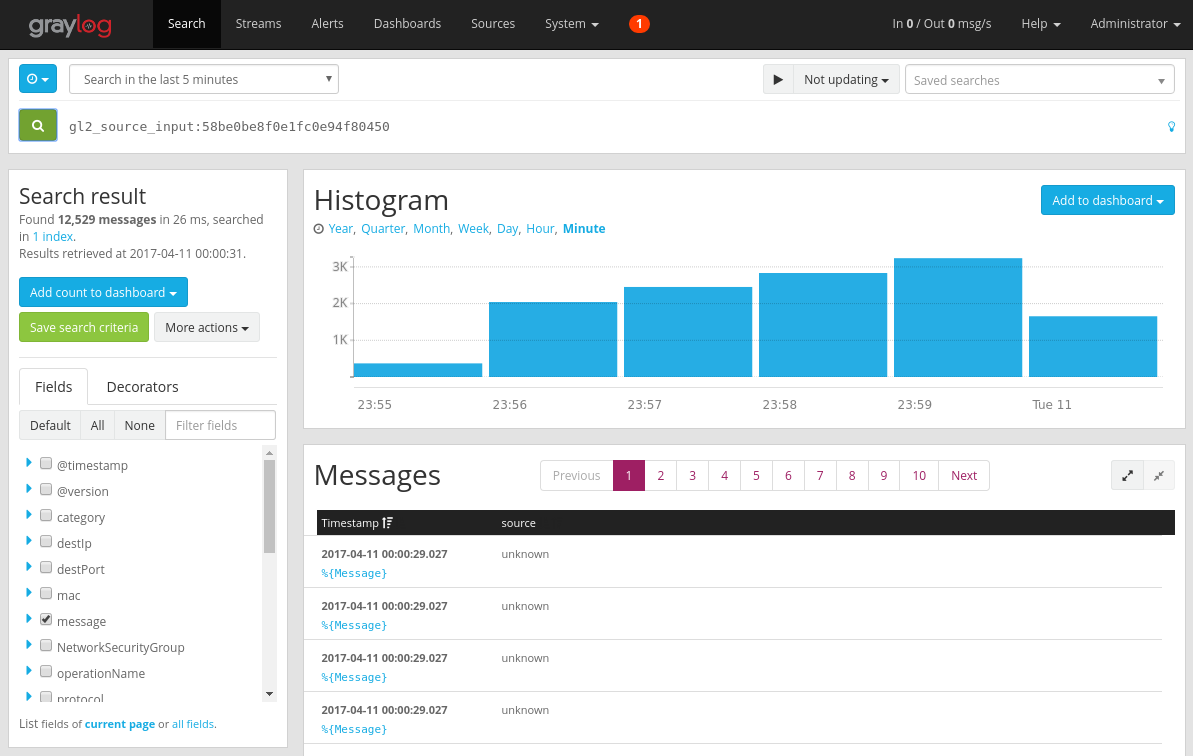
\includegraphics[width=0.85\textwidth]{images/img-024.png}
    \caption{Diagramme de cas d'utilisation de la plateforme cloud}
    \label{fig:use-case}
\end{figure}

\subsection{Diagramme de Classes}

\begin{figure}[H]
    \centering
    
\includegraphics[width=0.9\textwidth]{images/img-025.png}
    \caption{Diagramme de classes de la plateforme cloud}
    \label{fig:class-diagram}
\end{figure}

\subsection{Diagramme de Séquence}

\begin{figure}[H]
    \centering
    
\includegraphics[width=0.9\textwidth]{images/img-026.png}
    \caption{Diagramme de séquence pour le provisionnement IaaS}
    \label{fig:sequence-diagram}
\end{figure}

\newpage

% ============================================
% CHAPITRE 4
% ============================================
\chapter{Automatisation Cloud, Orchestration \& Monitoring (Sprints 2, 3, 4)}

\section{Sprint 2 : Automatisation de Cloud}

\subsection{Objectifs du Sprint}

\begin{itemize}
    \item Déployer OpenStack avec Kolla-Ansible
    \item Configurer Kubernetes sur OpenStack
    \item Intégrer Rancher pour la gestion multi-cluster
\end{itemize}

\subsection{Architecture de l'infrastructure déployée}

\begin{figure}[H]
    \centering
    
\includegraphics[width=0.9\textwidth]{images/img-027.png}
    \caption{Architecture OpenStack/Kubernetes}
    \label{fig:arch-openstack-k8s}
\end{figure}

\subsection{Installation d'OpenStack avec Kolla-Ansible}

\begin{lstlisting}[language=bash,caption={Installation OpenStack}]
# Installation des dependances
pip install kolla-ansible

# Configuration
cp -r /usr/share/kolla-ansible/etc_examples/kolla/* /etc/kolla/

# Deploiement
kolla-ansible -i multinode bootstrap-servers
kolla-ansible -i multinode prechecks
kolla-ansible -i multinode deploy
\end{lstlisting}

\subsection{Déploiement du cluster Kubernetes avec Ansible}

\begin{figure}[H]
    \centering
    
\includegraphics[width=0.85\textwidth]{images/img-028.png}
    \caption{OpenStack Infrastructure}
    \label{fig:openstack-infra}
\end{figure}

\subsection{Déploiement de Rancher sur OpenStack}

\begin{figure}[H]
    \centering
    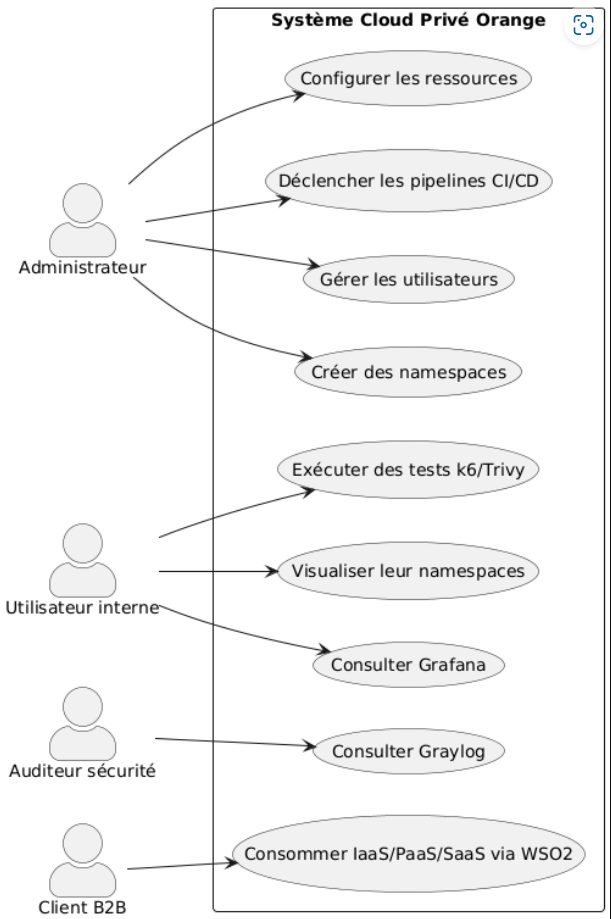
\includegraphics[width=0.85\textwidth]{images/img-030.png}
    \caption{Architecture Rancher et K8s sur OpenStack}
    \label{fig:rancher-k8s}
\end{figure}

\section{Sprint 3 : Orchestration des workflows OSS avec Camunda}

\begin{figure}[H]
    \centering
    
\includegraphics[width=0.9\textwidth]{images/img-031.png}
    \caption{Workflow BPMN pour résolution de panne OSS}
    \label{fig:bpmn-workflow}
\end{figure}

\section{Sprint 4 : Supervision avec Prometheus et Grafana}

\subsection{Collecte des métriques avec Prometheus}

Configuration de Prometheus pour collecter les métriques des différents composants.

\subsection{Dashboards Grafana}

\begin{figure}[H]
    \centering
    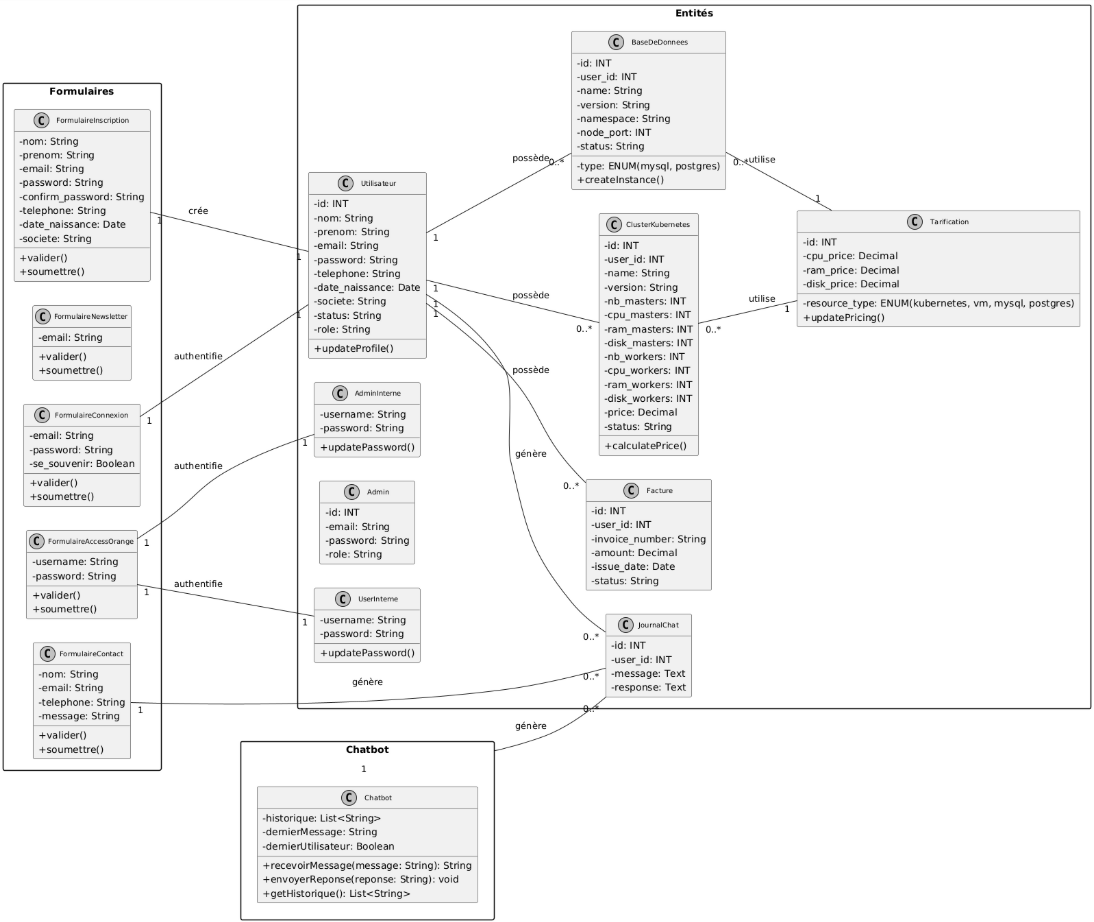
\includegraphics[width=0.9\textwidth]{images/img-032.png}
    \caption{Dashboard Grafana pour la supervision OSS}
    \label{fig:grafana-dashboard}
\end{figure}

\subsection{Alerting et scénarios d'incidents}

Configuration des alertes pour les indicateurs critiques :
\begin{itemize}
    \item CPU > 80\%
    \item Mémoire > 85\%
    \item Latence > 500ms
    \item Taux d'erreur > 5\%
\end{itemize}

\newpage

% ============================================
% CHAPITRE 5
% ============================================
\chapter{CI/CD, Gouvernance et Sécurité (Sprints 5, 6, 7)}

\section{Automatisation CI/CD et Gouvernance}

\subsection{Architecture Générale}

\begin{figure}[H]
    \centering
    
\includegraphics[width=0.9\textwidth]{images/img-033.png}
    \caption{Architecture de la plateforme DevSecOps}
    \label{fig:devsecops-arch}
\end{figure}

\subsection{Gestion des Namespaces et Permissions}

\begin{figure}[H]
    \centering
    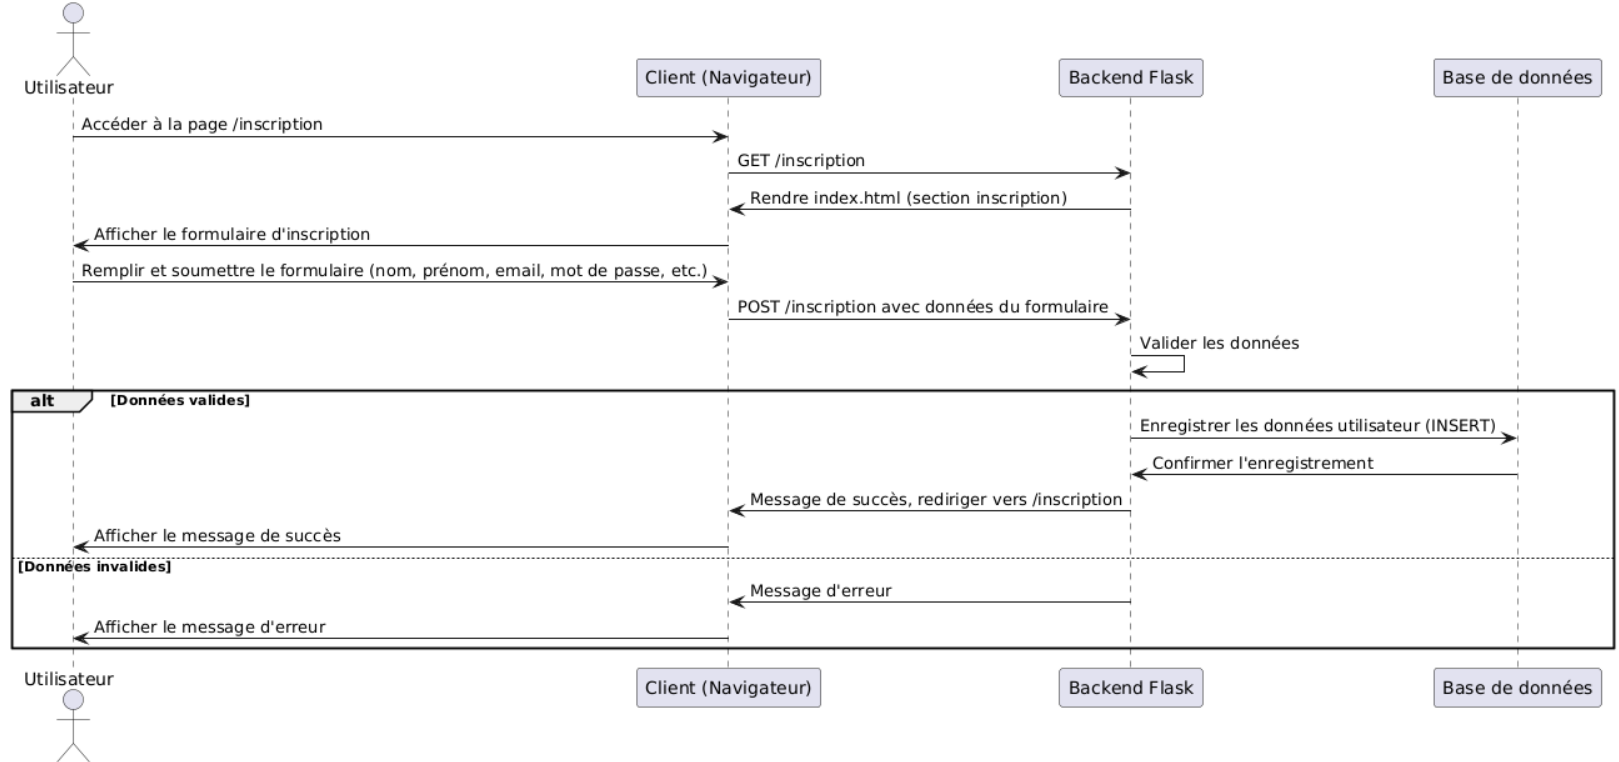
\includegraphics[width=0.7\textwidth]{images/img-034.png}
    \caption{Interface namespace}
    \label{fig:namespace-interface}
\end{figure}

\subsection{Automatisation CI/CD avec GitLab}

\begin{figure}[H]
    \centering
    
\includegraphics[width=0.8\textwidth]{images/img-035.png}
    \caption{Workflow d'automatisation CI/CD via Flask}
    \label{fig:cicd-workflow}
\end{figure}

\subsubsection{Détection Automatique du Langage}

Le système détecte automatiquement le langage de programmation utilisé.

\subsubsection{Génération Automatique des Fichiers}

Génération automatique des fichiers de configuration (Dockerfile, .gitlab-ci.yml).

\subsubsection{Exécution et Déploiement}

Pipeline complet de build, test et déploiement.

\section{Sécurité Offensive et Défensive}

\subsection{Pentest avec KubeHunter}

\begin{figure}[H]
    \centering
    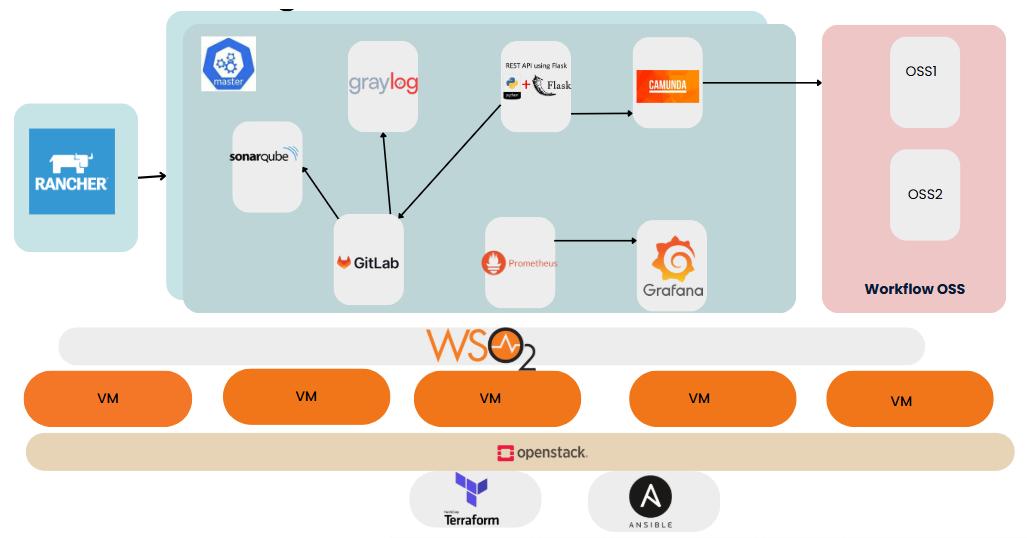
\includegraphics[width=0.8\textwidth]{images/img-036.png}
    \caption{Scan KubeHunter sur Kubernetes}
    \label{fig:kubehunter-scan}
\end{figure}

\subsection{Centralisation des Logs avec Graylog}

\subsubsection{Logs et Sécurité dans Kubernetes}

Collecte centralisée de tous les logs du cluster.

\subsubsection{Déploiement de Graylog}

\begin{lstlisting}[language=yaml,caption={Déploiement Graylog}]
apiVersion: apps/v1
kind: Deployment
metadata:
  name: graylog
spec:
  replicas: 1
  template:
    spec:
      containers:
      - name: graylog
        image: graylog/graylog:5.0
        ports:
        - containerPort: 9000
\end{lstlisting}

\begin{figure}[H]
    \centering
    
\includegraphics[width=0.9\textwidth]{images/img-037.png}
    \caption{Dashboard Graylog pour K8s}
    \label{fig:graylog-dashboard}
\end{figure}

\section{Interface Utilisateur et Automatisations}

Interface web développée avec Flask pour la gestion centralisée de la plateforme.

\newpage

% ============================================
% CHAPITRE 6
% ============================================
\chapter{Offres B2B – IaaS, PaaS, SaaS (Sprint 8)}

\section{Offre IaaS – Infrastructure as a Service}

\subsection{Description du Service}

L'offre IaaS permet aux clients de provisionner des machines virtuelles sur demande.

\begin{table}[H]
    \centering
    \caption{Offres IaaS}
    \label{tab:iaas}
    \rowcolors{2}{lightgray}{white}
    \begin{tabular}{|l|c|c|c|c|}
        \hline
        \rowcolor{orange!80}
        \textcolor{white}{\textbf{Offre}} & \textcolor{white}{\textbf{vCPU}} & \textcolor{white}{\textbf{RAM}} & \textcolor{white}{\textbf{Stockage}} & \textcolor{white}{\textbf{Prix/mois}} \\
        \hline
        Small & 2 & 4 Go & 50 Go & 50 DT \\
        Medium & 4 & 8 Go & 100 Go & 100 DT \\
        Large & 8 & 16 Go & 200 Go & 200 DT \\
        XLarge & 16 & 32 Go & 500 Go & 400 DT \\
        \hline
    \end{tabular}
\end{table}

\subsection{Processus de Provisionnement}

\begin{enumerate}
    \item Le client sélectionne l'offre souhaitée
    \item Validation et paiement
    \item Provisionnement automatique via OpenStack
    \item Notification et accès remis au client
\end{enumerate}

\subsection{Cas d'Usage Client}

\begin{itemize}
    \item Hébergement de sites web
    \item Environnements de développement
    \item Tests et staging
\end{itemize}

\section{Offre PaaS – Platform as a Service}

\subsection{Déploiement de Clusters Kubernetes}

Les clients peuvent déployer leurs propres clusters Kubernetes managés.

\subsection{Bases de Données MySQL \& PostgreSQL}

Bases de données managées avec backup automatique.

\begin{table}[H]
    \centering
    \caption{Offres bases de données}
    \label{tab:bdd}
    \rowcolors{2}{lightgray}{white}
    \begin{tabular}{|l|c|c|c|}
        \hline
        \rowcolor{orange!80}
        \textcolor{white}{\textbf{Type}} & \textcolor{white}{\textbf{RAM}} & \textcolor{white}{\textbf{Stockage}} & \textcolor{white}{\textbf{Prix/mois}} \\
        \hline
        MySQL Small & 2 Go & 20 Go & 30 DT \\
        MySQL Medium & 4 Go & 50 Go & 60 DT \\
        PostgreSQL Small & 2 Go & 20 Go & 35 DT \\
        PostgreSQL Medium & 4 Go & 50 Go & 70 DT \\
        \hline
    \end{tabular}
\end{table}

\subsection{Interface de Consommation}

Interface web pour la gestion des services PaaS.

\section{Offre SaaS – Security \& Services as a Service}

\subsection{Web Application Firewall (WAF)}

Protection des applications web contre les attaques courantes (SQL injection, XSS, etc.).

\section{Économie et Gestion pour Clients Multiples}

\subsection{Modèle Économique}

Modèle pay-as-you-go avec facturation mensuelle.

\subsection{Gestion pour Clients Multiples}

\begin{itemize}
    \item Isolation par namespace Kubernetes
    \item Quotas de ressources par client
    \item Facturation automatisée
    \item Support multi-tenant
\end{itemize}

\newpage

% ============================================
% CONCLUSION
% ============================================
\chapter*{Conclusion Générale}
\addcontentsline{toc}{chapter}{Conclusion Générale}

Ce projet de fin d'études a permis de concevoir et déployer une plateforme cloud complète pour Orange Tunisie, intégrant :

\begin{itemize}
    \item \textbf{OpenStack} pour la virtualisation IaaS
    \item \textbf{Kubernetes} pour l'orchestration des conteneurs
    \item \textbf{Rancher} pour la gestion multi-cluster
    \item \textbf{GitLab CI/CD} pour l'automatisation des déploiements
    \item \textbf{Prometheus/Grafana} pour le monitoring
    \item \textbf{Graylog} pour la centralisation des logs
    \item Des \textbf{offres B2B} (IaaS, PaaS, SaaS)
\end{itemize}

La méthodologie Scrum a permis une approche incrémentale et itérative, facilitant l'adaptation aux évolutions des besoins.

\textbf{Perspectives d'amélioration :}
\begin{itemize}
    \item Intégration de l'IA pour la prédiction des incidents
    \item Extension des offres SaaS
    \item Amélioration de la haute disponibilité
    \item Certification ISO 27001
\end{itemize}

\newpage

% ============================================
% BIBLIOGRAPHIE
% ============================================
\chapter*{Bibliographie}
\addcontentsline{toc}{chapter}{Bibliographie}

\begin{enumerate}
    \item \textbf{OpenStack Documentation} - \url{https://docs.openstack.org/}
    \item \textbf{Kubernetes Documentation} - \url{https://kubernetes.io/docs/}
    \item \textbf{Rancher Documentation} - \url{https://rancher.com/docs/}
    \item \textbf{GitLab CI/CD} - \url{https://docs.gitlab.com/ee/ci/}
    \item \textbf{Prometheus} - \url{https://prometheus.io/docs/}
    \item \textbf{Grafana} - \url{https://grafana.com/docs/}
    \item \textbf{Graylog} - \url{https://docs.graylog.org/}
    \item \textbf{Terraform} - \url{https://www.terraform.io/docs/}
    \item \textbf{Ansible} - \url{https://docs.ansible.com/}
    \item \textbf{Camunda} - \url{https://docs.camunda.io/}
\end{enumerate}

\end{document}
